\documentclass[12pt]{article}
\usepackage{float}
\usepackage[table,xcdraw]{xcolor}
\usepackage{tikzit}
\input{Homework.tikzstyles}
\usepackage{hyperref}
\usepackage{amsmath}
\usepackage{amsfonts}
\usepackage{amssymb}
\usepackage{amsthm}
\usepackage{graphics}
\usepackage{graphicx}
\usepackage{yfonts}
\usepackage{float}
\usepackage[textwidth=17cm, textheight=24cm]{geometry}
\usepackage{dsfont}
\usepackage[nottoc]{tocbibind}
\setcounter{tocdepth}{3}
\setcounter{secnumdepth}{3}
\usepackage{url}
\usepackage{multirow}
\usepackage{subcaption}
\usepackage{caption}
\usepackage[font=scriptsize]{caption}
\usepackage{ctable}
\usepackage{caption}
\usepackage{pifont}
\usepackage{array}
\usepackage{multirow}
\usepackage{subcaption}
\usepackage{ctable}
\usepackage{adjustbox}
\usepackage{booktabs}
\usepackage{tabularx, booktabs, makecell, caption}
\usepackage{siunitx}
\usepackage{booktabs}
\usepackage{xepersian}
\settextfont[
BoldFont=XB ZarBd.TTF,
ItalicFont=XB ZarIt.TTF,
BoldItalicFont=XB ZarBdIt.TTF]{XB Zar.TTF}
\ExplSyntaxOn \cs_set_eq:NN \etex_iffontchar:D \tex_iffontchar:D \ExplSyntaxOff
\setdigitfont[
BoldFont=XB ZarBd.TTF,
ItalicFont=XB ZarIt.TTF,
BoldItalicFont=XB ZarBdIt.TTF]{XB Zar.TTF}

\title{\Luge پروژه دوم درس علوم اعصاب محاسباتی\\[1ex]آشنایی با عملکرد سیناپس‌ها و جمعیت‌های نورونی}
\author{\\ \Large{ محمد زمانی}  \\ \\ \Large{شماره دانشجویی: ۶۱۰۳۹۹۱۳۵} \\ \\ }}
\date{}

\usepackage{titling}
\renewcommand\maketitlehooka{\null\mbox{}\vfill}
\renewcommand\maketitlehookd{\vfill\null}

\begin{document}
	%%%%%%%%%%%%%%%%%%%%%       Title Page      %%%%%%%%%%%%%%%%%%%%%%		

	
	\begin{titlingpage}
	
	\begin{figure}
		\centering
		
\includegraphics[width=0.3\textwidth]{Figs/University_of_Tehran_logo.png}	
		\caption*{ \LARGE دانشگاه تهران\\ دانشکده ریاضی و علوم کامپیوتر \\}
	\end{figure}	\maketitle
	
	\end{titlingpage}

	%%%%%%%%%%%%%%%%%%%%%       Page 1       %%%%%%%%%%%%%%%%%%%%%%

	\setlength{\parindent}{20pt}
	\tableofcontents
	
	\vspace{1\baselineskip}

	\pagebreak
	\section{مقدمه}
	می‌دانیم که مدل‌های مختلفی برای تک نورون وجود دارد که در پروژه قبل آن‌ها را بررسی و تحلیل کردیم
، اما همانطور که می‌دانیم مغز ما از میلیاردها نورون تشکیل شده است که اینها به صورت سلسله مراتبی در نواحی مختلف مغز قرار گرفتەاند که می‌توان همه آنها را به صورت جمعیتهای
نورونی دید، بنابراین مطالعه جمعیت‌های نورونی اهمیت بسزایی دارد. در این پروژه می‌خواهیم رفتار جمعیت‌های نورونی و الگو‌های ارتباطی میان‌ آن‌ها و همچنین فرآیند تصمیم گیری را مورد بحث و تحلیل قرار دهیم.

	\section{سیناپس}
	
	\subsection{ فضای سیناپسی}
	

اگر که یک نورون \lr{presynoptic}
فعال شود این فعالیت از طریق فضایی به نام سیناپس به نورون \lr{postsynaptic}	
منتقل می‌شود. وقتی که نورون \lr{presynaptic} فعال می‌شود این فعالیت به انتهای \lr{axon} می‌رسد که به آن ها \lr{terminal buttom}	
می‌گویند، اینها باعث می‌شود که \lr{vesicle} ها به سمت جلو حرکت کنند و برخی از آن‌ها نزدیک غشای نورونی می‌شوند و می‌چسبند به غشا و محتویات خودشان را که \lr{neurotransmitter} ها است در فضای سیناپسی آزاد می‌کنند، در این فضا کانال های یونی وجود دارد که این \lr{neurotransmitter} ها می‌چسبند به دریافت کننده ها و این کانال های یونی باز می‌شوند و با توجه به اینکه نورون ما مهاری است یا تحریکی پتاسیم یا سدیم وارد نورون می‌شود، شمای کلی این فرآیند را می‌توانید در شکل \ref{Fig:syn} ببینید.

\begin{figure}[H]
\centering
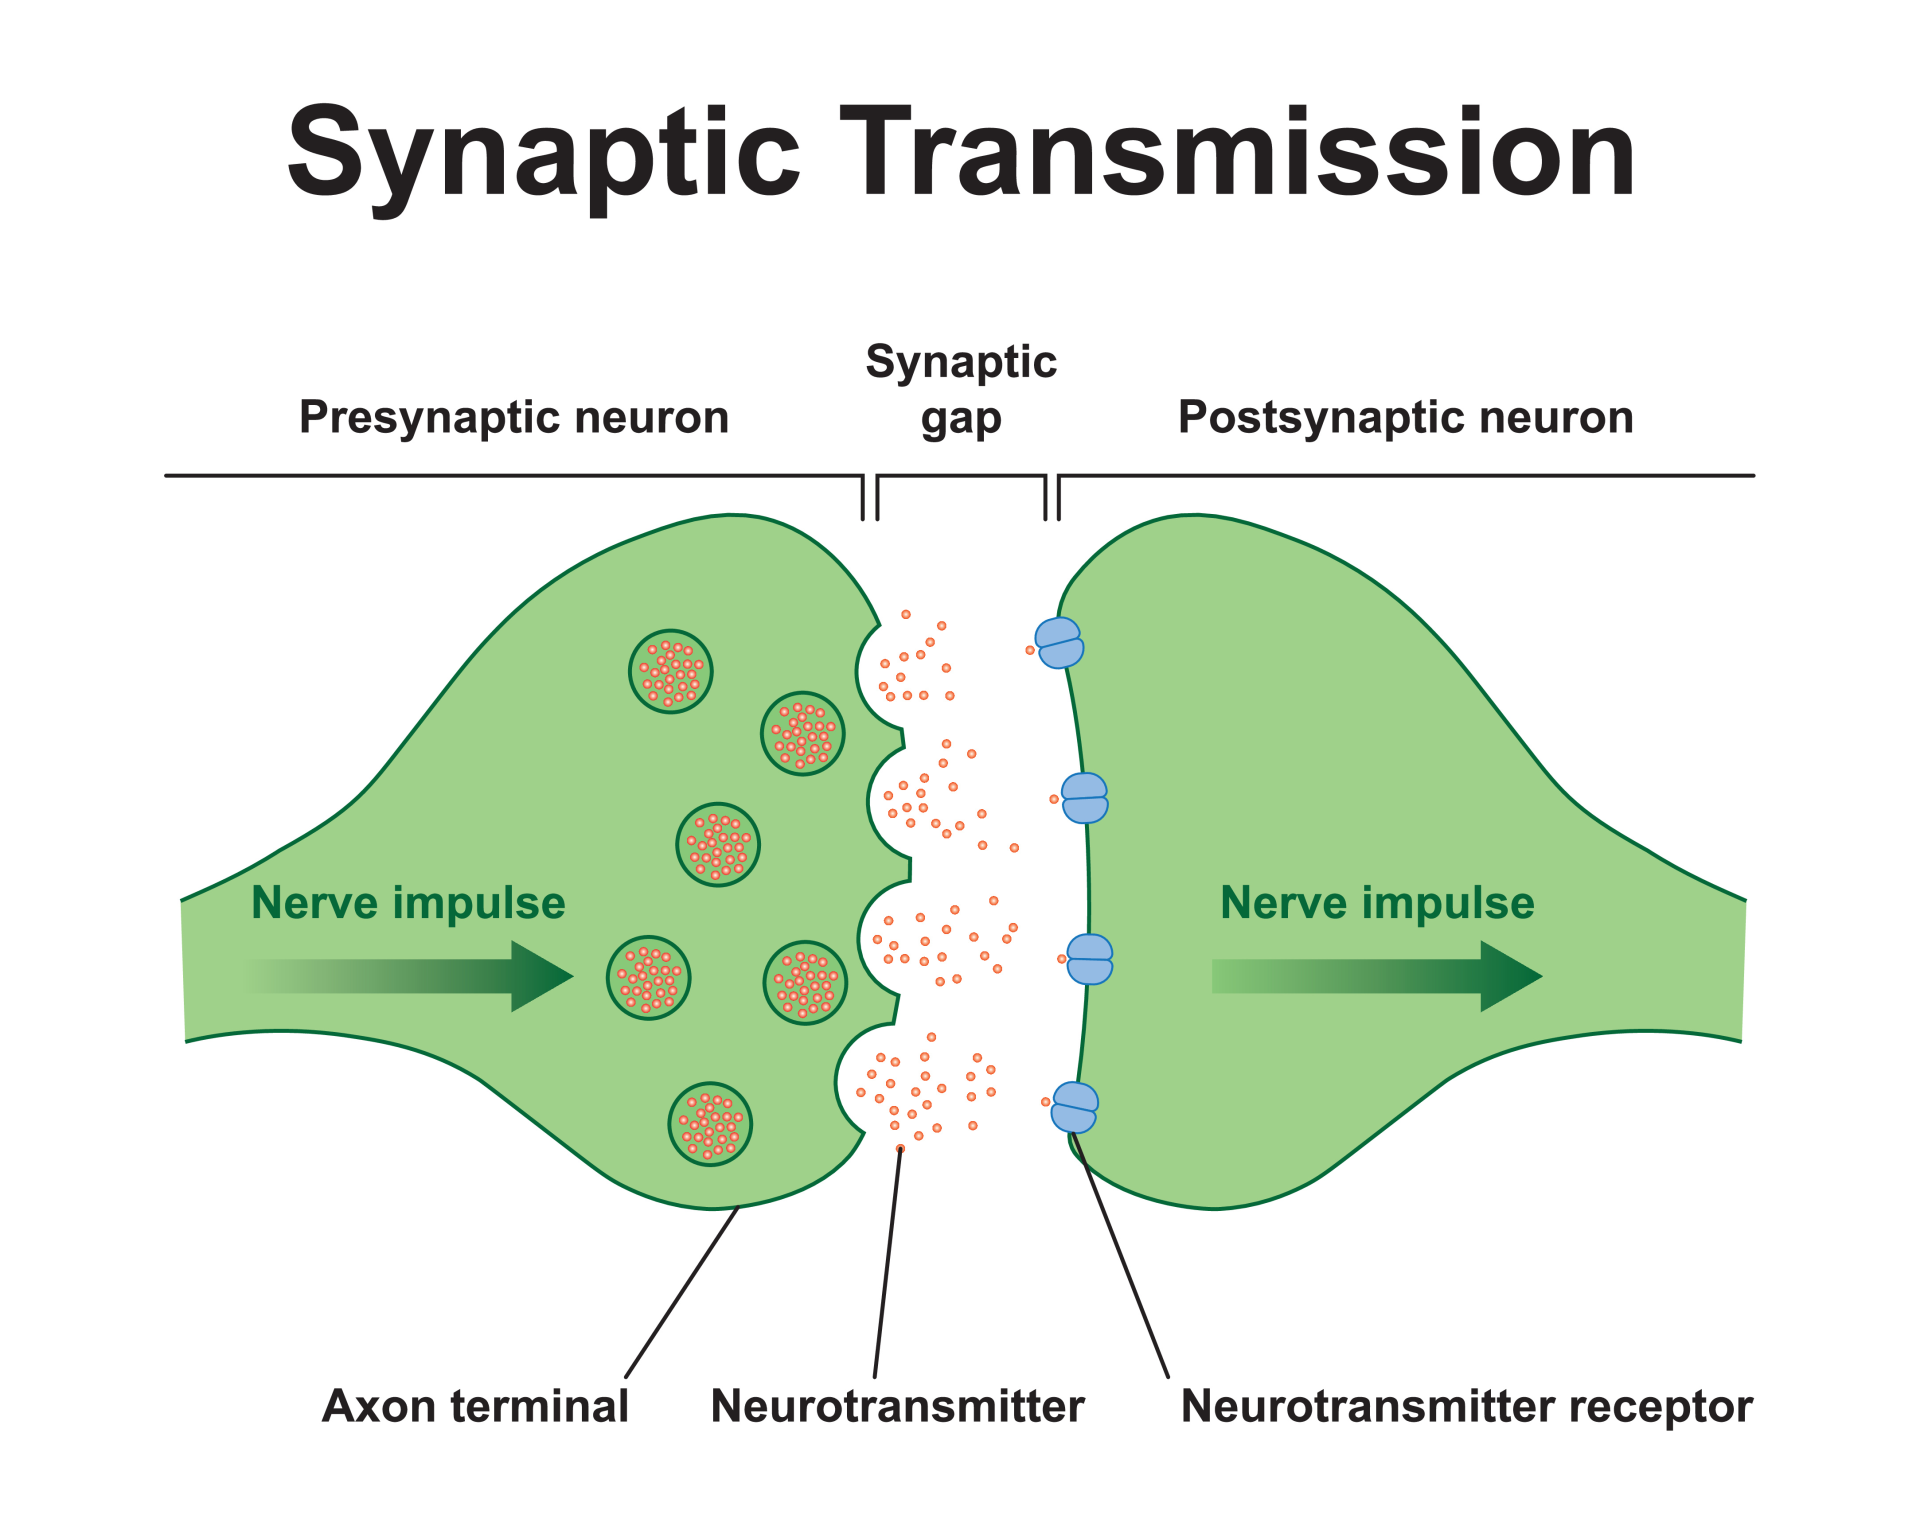
\includegraphics[width=5.5cm]{Figs/Chemical-synapse.png}
\caption{انتقال سیناپسی}
\label{Fig:syn}
\end{figure}
\end{center}

همانطور که در شکل \ref{Fig:syn} مشاهده می‌کنید فعالیت نورون ها در فضای سیناپسی از طریق کانال های یونی منتقل می‌شود و به هر میزان تعداد این کانال های یونی بیشتر باشند میزان اثر گذاری نورون قبلی بر روی نورون بعدی بیشتر خواهد بود، اصولا چیزی که ما به آن یادگیری می‌گوییم همین میزان اثر گذاری فعالیت یک نورون بر روی نورون بعدی است که میزان کم یا زیاد شدن اثر گذاری نورون \lr{presynaptic} بر روری نورون \lr{postsynaptic} را \lr{synaptic placity} می‌گویند.


	\subsection{شبیه‌سازی سیپناپس با استفاده از تابع دلتای دیراک}
	در این بخش با استفاده از این  تابع می‌خواهیم سازوکار سیناپس را مدل کنیم.
تابع دلتای دیراک به این صورت است که به صورت یکنواخت مقدار صفر دارد، به جز نقطه صفر، به طوری که روی کل محور اعداد حقیقی انتگرال آن برابر است با یک که می‌توان رفتار این تابع را در شکل \ref{fig:DDF}  مشاهده نمود.

\begin{figure}[H]
\centering
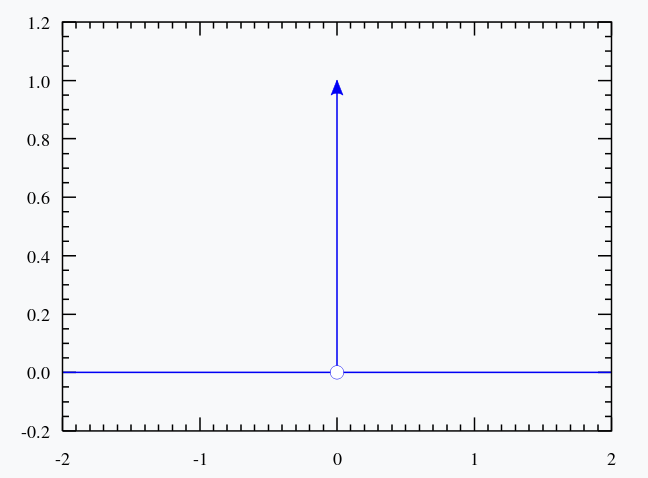
\includegraphics[width=0.4\textwidth]{Figs/DDF}
\caption{نمایش شماتیک تابع دلتا دیراک}
\label{fig:DDF}
\end{figure}
\end{center}

حال در مدل‌سازی رفتار سیناپس ها با استفاده از این تابع به این صورت عمل می‌کنیم که زمان هایی که نورون‌های پیشین	\LTRfootnote{pre-synaptic neuron}
ضربه ‌می‌زنند در یک لحظه بر روی نورون‌های بعدی اثر می‌گذارند که این ساده‌ترین مدلی است که می‌توان برای سیناپس ارائه داد.

به عنوان مثال ما یک جمعیت نورونی که متشکل از هزار نورون \lr{LIF} است را به یک جمعیت نورونی که متشکل از یک نورون \lr{LIF} است متصل می‌کنیم، هیچ اتصالی میان نورون های‌ هر جمعیت وجود ندارد اما همه نورون‌های جمعیت اولیه به تک نورون جمعیت دوم متصل است، حال یک شبیه‌سازی با استفاده از سیناپس پیاده سازی شده انجام می‌دهیم.


\begin{figure}[H]
\centering
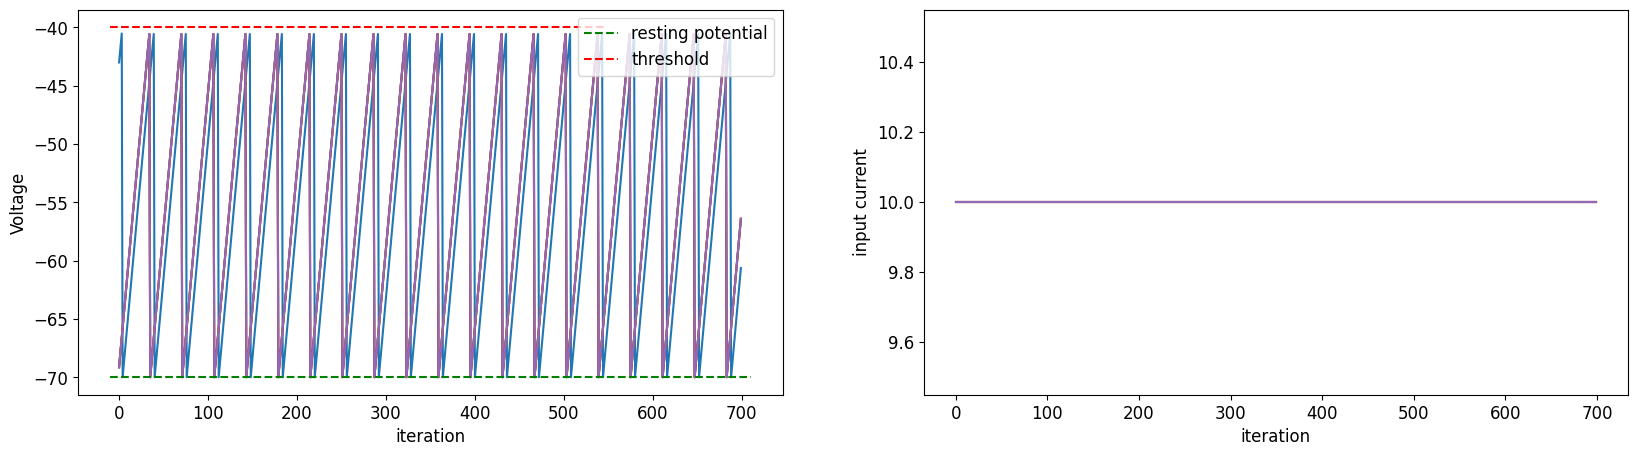
\includegraphics[width=0.9\textwidth]{Figs/NG1.png}
\caption{جریان ورودی و تغییرات پتانسیل پنج نورون تصادفی از جمعیت اول }
\label{fig:NG1}
\end{figure}
\end{center}


\begin{figure}[H]
\centering
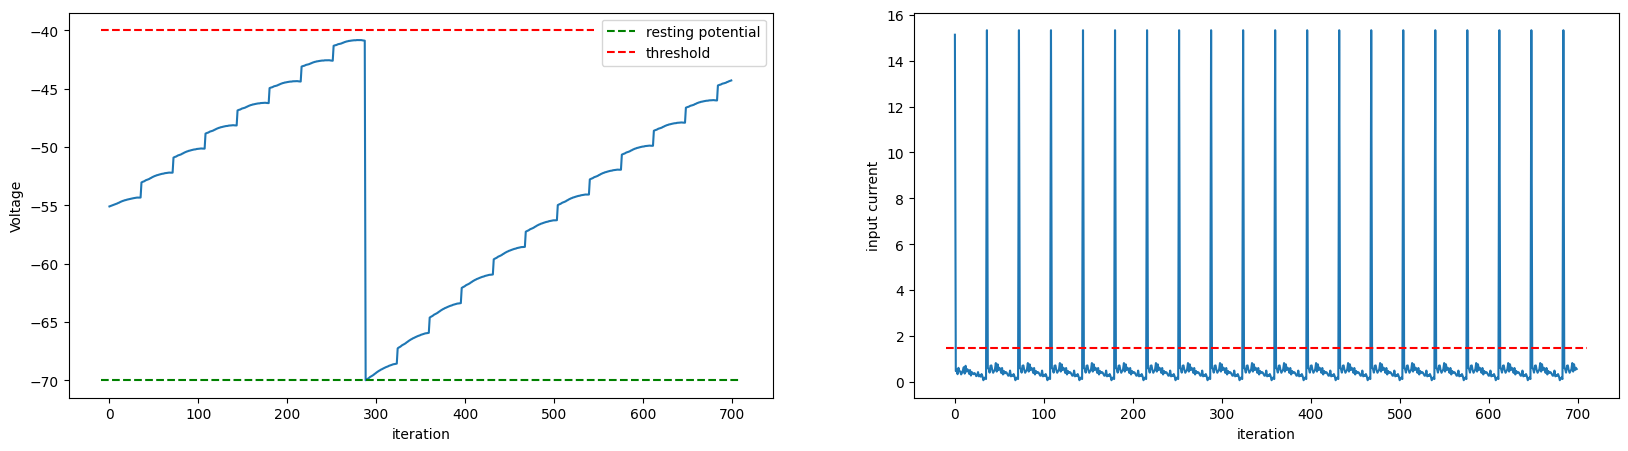
\includegraphics[width=0.9\textwidth]{Figs/NG2.png}
\caption{جریان ورودی و تغییرات پتانسیل تک نورون جمعیت دوم }
\label{fig:NG2}
\end{figure}
\end{center}


همانطور که در شکل \ref{fig:NG1} مشاهده می‌کنید به همه نورون‌های جمعیت اول یک جریان ثابت ۱۰ آمپری وارد می‌شود که تغییرات اختلاف پتانسیل پنج‌ تا از نورون‌ها نیز در شکل آمده است، حال به تک نورون جمعیت دوم هیچ جریان ورودی ثابتی داده نمی‌شود و فقط از طریق سیناپس جریان ورودی به آن منتقل می‌شود، همانطور که نمودار تغییرات جریان را در شکل \ref{fig:NG2} مشاهده ‌می‌کنید، زمان‌هایی که نورون‌های جمعیت اول ضربه می‌زنند، جریان ورودی به تک نورودن جمعیت دوم بیشینه می‌شود اما در بقیه موارد زمان‌ها اینگونه نیست، که این رفتار مطابق آن چیزی است که ما در مدل سازی تابع دلتا دیراک ادعا کرده بودیم، تنها وقتی که نورونی ضربه‌ می‌زند فعالیتش به نورون پسین منتقل می‌گردد، که این انتقال فعالیت را ما با انتقال جریان از طریق سیناپس‌ها مدل می‌کنیم.


حال همین آزمایشات را با استفاده از مدل نورونی \lr{ELIF} نیز انجام می‌دهیم.


\begin{figure}[H]
\centering
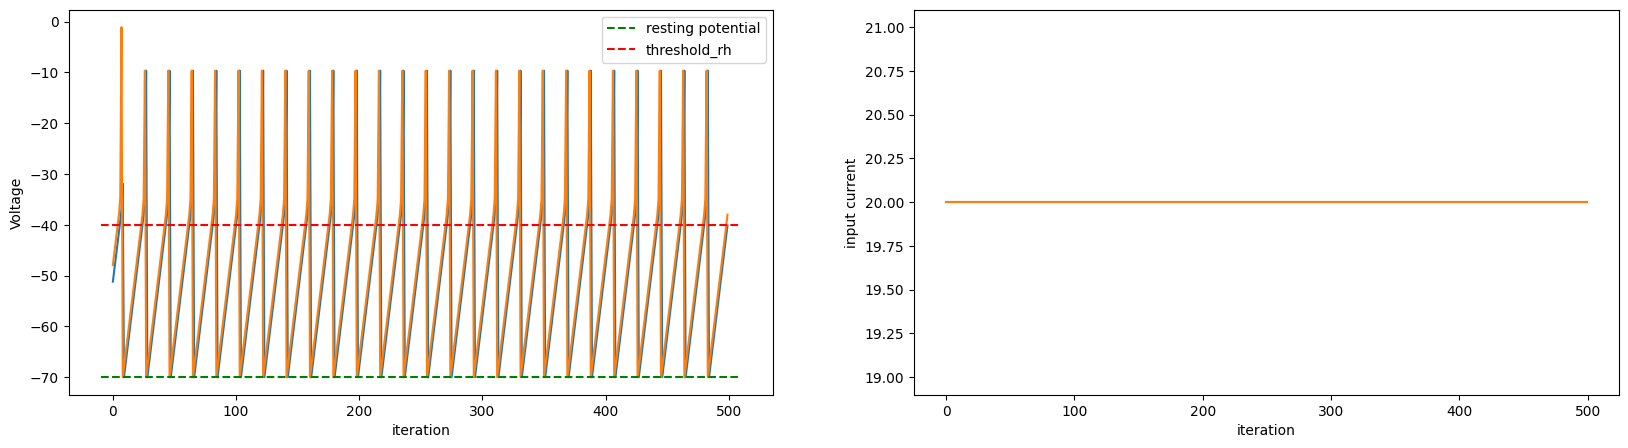
\includegraphics[width=0.9\textwidth]{Figs/NG1E.png}
\caption{جریان ورودی و تغییرات پتانسیل دو نورون تصادفی از جمعیت اول }
\label{fig:NG1E}
\end{figure}
\end{center}


\begin{figure}[H]
\centering
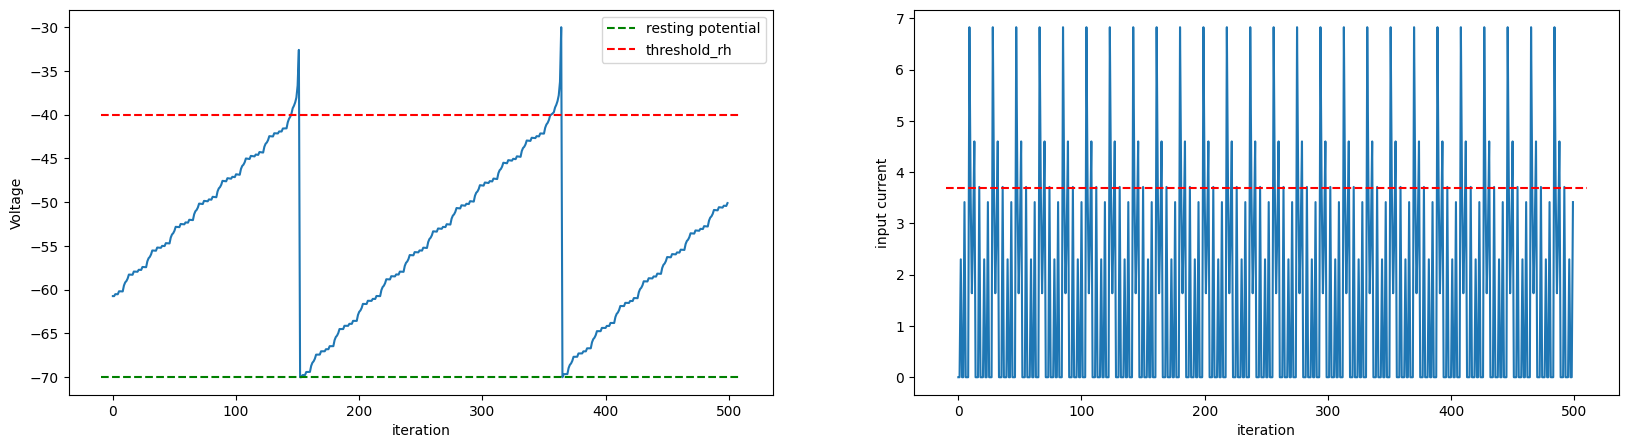
\includegraphics[width=0.9\textwidth]{Figs/NG2E.png}
\caption{جریان ورودی و تغییرات پتانسیل تک نورون جمعیت دوم }
\label{fig:NG2E}
\end{figure}
\end{center}

همانطور که در شکل \ref{fig:NG2E} مشاهده می‌کنید، در این مدل نورونی پتانسیل فعالیت باعث می‌شود که به نوعی هر ضربه در طول بازه بزرگتری رخ دهد که این در جریان ورودی تک نورون ما در جمعیت دوم خود را نشان داده است، در بقیه موارد کاملا رفتار مشابهی هر دو مدل داشته‌اند.


\section{الگوهای ارتباطی}

در هر کدام از بخش‌ها یک جمعیت نورونی با صد نورون \lr{LIF} خواهیم داشت، که با الگوهای ارتباطی متفاوت میان نورون‌ها ارتباط برقرار می‌کنیم، سپس به هر کدام جریان بدون نویز و با نویز وارد می‌کنیم و عملکرد و فعالیت هر کدام از نورون‌ها را مقایسه می‌کنیم.

\subsection{\lr{full connectivity schema}}

در این حالت هر دو نورونی که در جمعیت نورنی وجود دارد بهم متصل هستند و برای وزن‌دهی نیز یک وزن ثابت $w_{ij} =  \frac{j_0}{N}$ میان هر دو نورون در نظر میگیریم یا اینکه وزن‌دهی با استفاده از یک توزیع گاوسی با میانگین $m = \frac{j_0}{N}$ و واریانس $\frac{\phi_0}{N}$ انجام می‌شود.


\begin{figure}[H]
\centering
  \begin{subfigure}[b]{0.9\textwidth}
    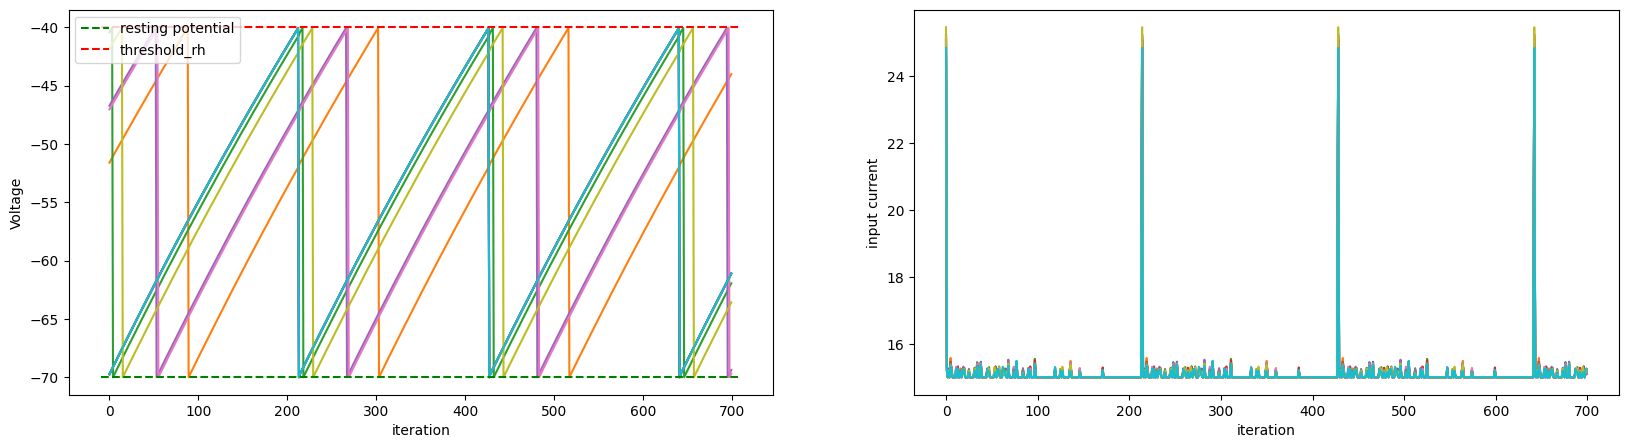
\includegraphics[width=\textwidth]{Figs/full_v.png}
    \caption{جریان ورودی بدون نویز}
  \end{subfigure}
  \\[\smallskipamount]
  \begin{subfigure}[b]{0.9\textwidth}
    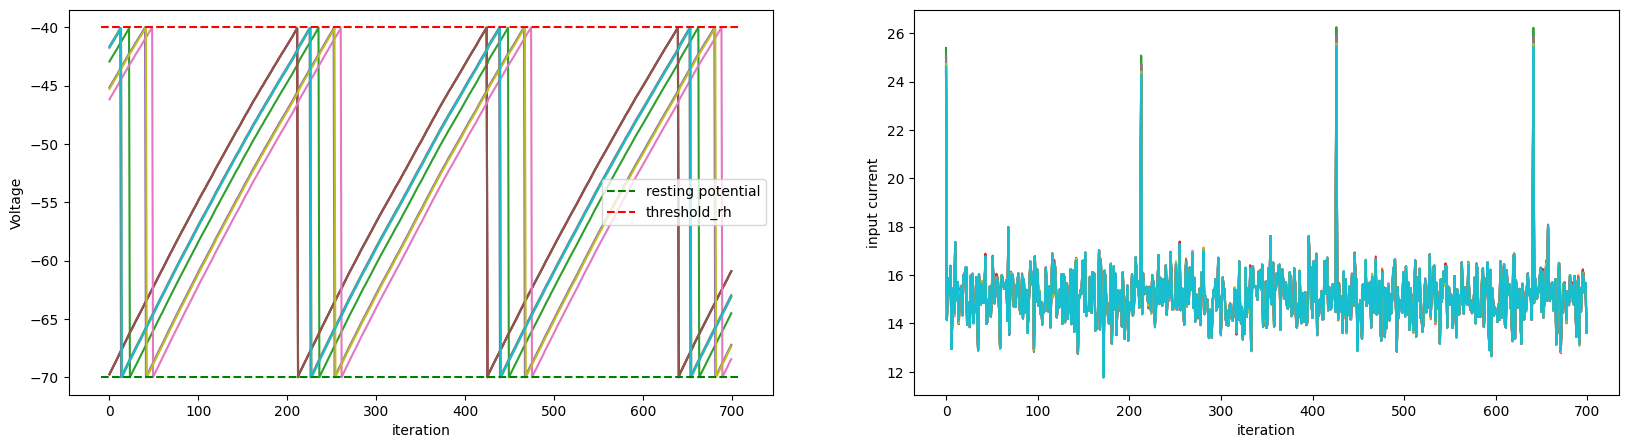
\includegraphics[width=\textwidth]{Figs/full_n_v.png}
    \caption{جریان ورودی با نویز}
  \end{subfigure}
  \caption{مقایسه تغییرات پتانسیل نورون با جریان ورودی نویزی و بدون نویز}
  \label{Fig:compare}
\end{figure}
\end{center}




\subsection{\lr{fixed coupling probability}}

در این حالت از میان $N^2$
حالت ممکن برای ایجاد ارتباط با احتمال ثابت $p$ از میان آن‌ها انتخاب انجام می‌دهیم و وزن را قرار می‌دهیم 	
.$w_{ij} = \frac{j_0}{pN}$



\begin{figure}[H]
\centering
  \begin{subfigure}[b]{0.9\textwidth}
    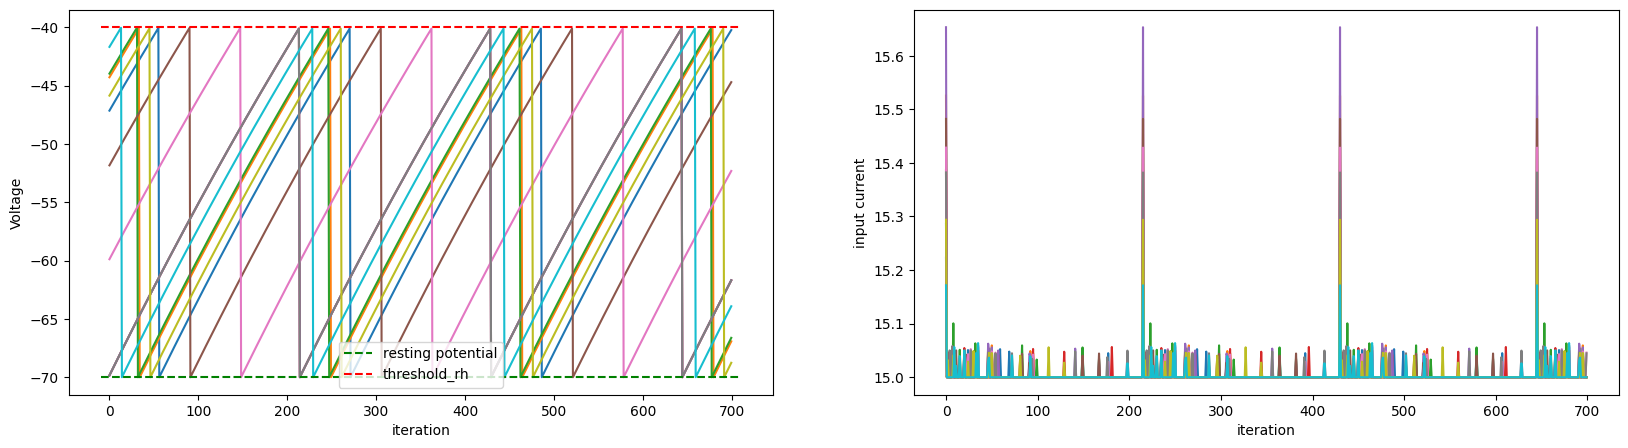
\includegraphics[width=\textwidth]{Figs/fixed_prob_v.png}
    \caption{جریان ورودی بدون نویز}
  \end{subfigure}
  \\[\smallskipamount]
  \begin{subfigure}[b]{0.9\textwidth}
    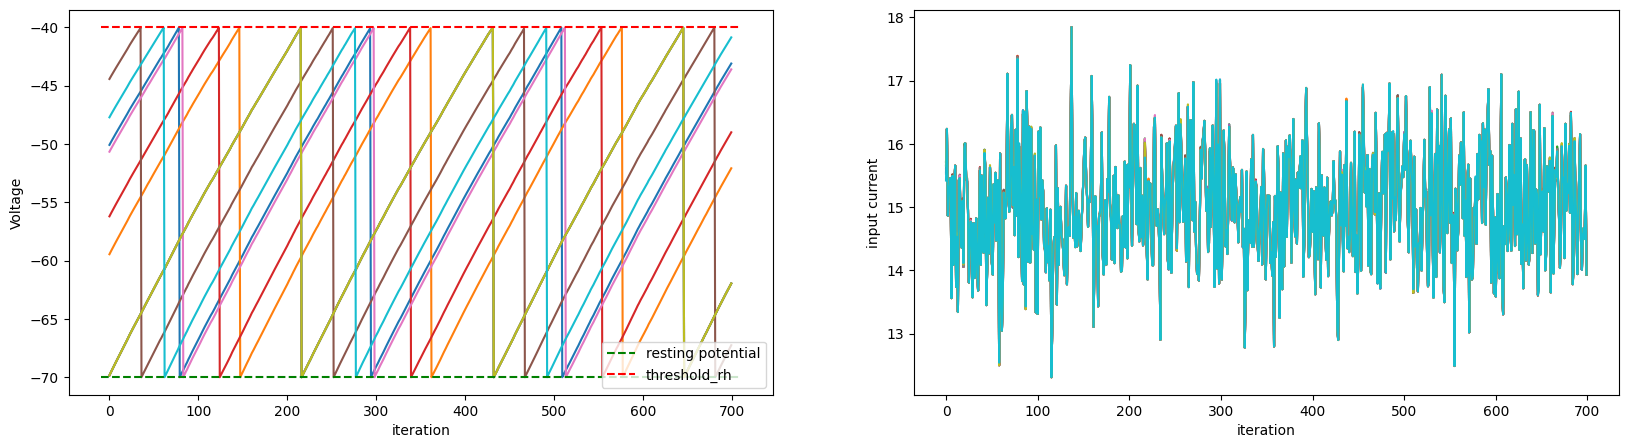
\includegraphics[width=\textwidth]{Figs/fixed_prob_v_n.png}
    \caption{جریان ورودی با نویز}
  \end{subfigure}
  \caption{مقایسه تغییرات پتانسیل نورون با جریان ورودی نویزی و بدون نویز}
  \label{Fig:compare}
\end{figure}
\end{center}


\subsection{\lr{fixed number of presynaptic partners}}

در این حالت تعداد نورنی‌های متصل به یک نورون برای همه نورن‌ها مقداری ثابت خواهد بود اما اتصالات به صورت تصادفی خواهد بود همانند حالت قبل.

\begin{figure}[H]
\centering
  \begin{subfigure}[b]{0.9\textwidth}
    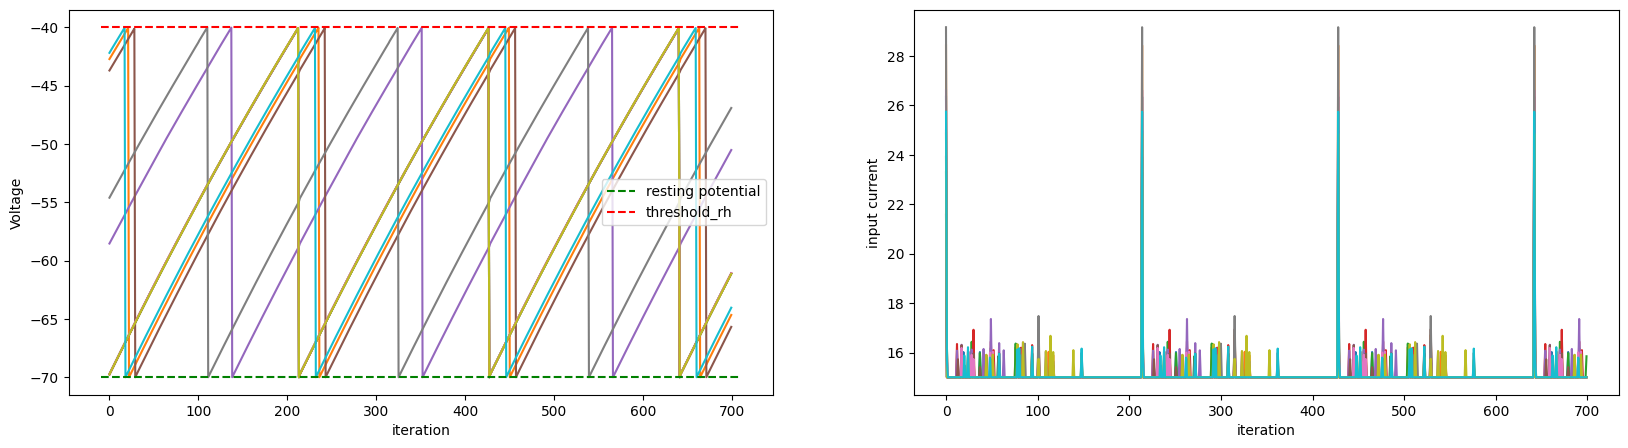
\includegraphics[width=\textwidth]{Figs/fixed_count_v.png}
    \caption{جریان ورودی بدون نویز}
  \end{subfigure}
  \\[\smallskipamount]
  \begin{subfigure}[b]{0.9\textwidth}
    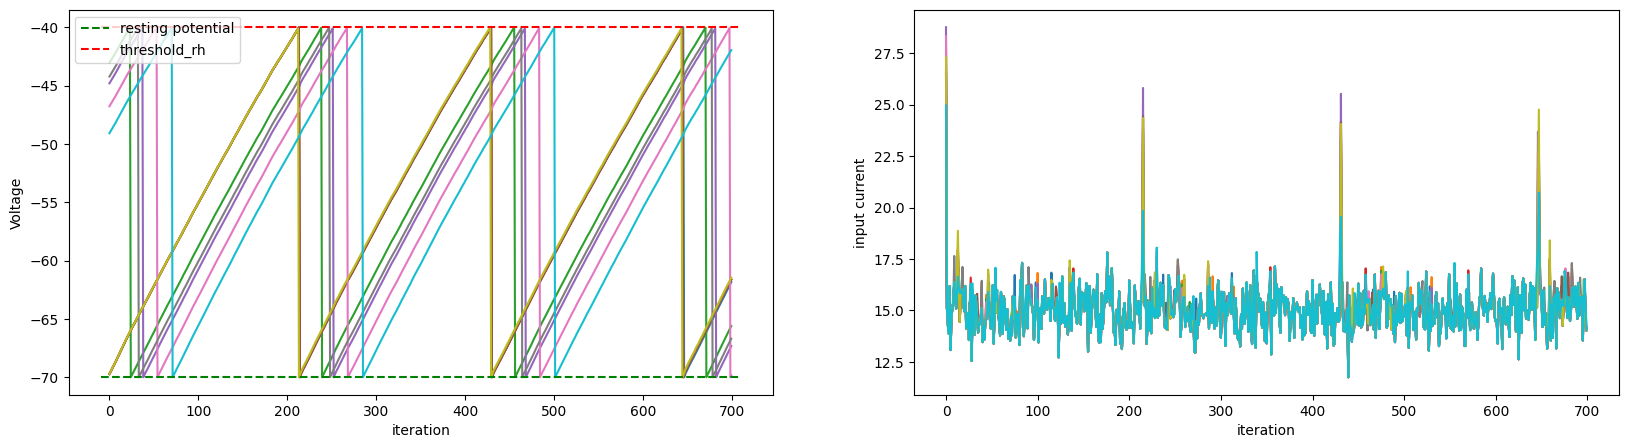
\includegraphics[width=\textwidth]{Figs/fixed_count_v_n.png}
    \caption{جریان ورودی با نویز}
  \end{subfigure}
  \caption{مقایسه تغییرات پتانسیل نورون با جریان ورودی نویزی و بدون نویز}
  \label{Fig:compare}
\end{figure}
\end{center}

\subsection{مقایسه الگوهای ارتباطی}
در نهایت تعداد ضربه‌های هر یک از نورون‌ها را در حالتی که جریان نویز دارد یا بدون نویز است شماردیم و نمودارهای آن را در شکل \ref{Fig:compare} می‌توان دید.

\begin{figure}[H]
  \begin{subfigure}[b]{0.3\textwidth}
    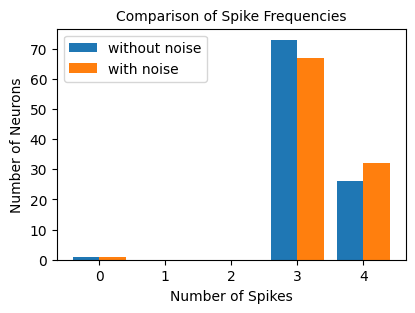
\includegraphics[width=\textwidth]{Figs/full.png}
    \caption{\lr{full connectivity schema}}
  \end{subfigure}
  \hfill
  \begin{subfigure}[b]{0.3\textwidth}
    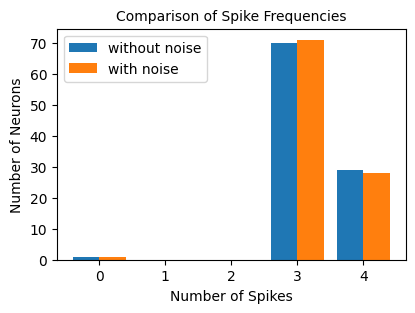
\includegraphics[width=\textwidth]{Figs/fixed_prob.png}
    \caption{\lr{fixed coupling probability}}
  \end{subfigure}
  \hfill
  \begin{subfigure}[b]{0.3\textwidth}
    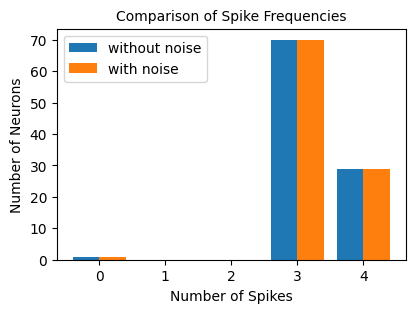
\includegraphics[width=\textwidth]{Figs/fixed_count.png}
    \caption{\lr{fixed number of presynaptic partners}}
  \end{subfigure}
  \caption{مقایسه حساسیت به نویز در الگوهای متفاوت ارتباطی}
  \label{Fig:compare}
\end{figure}


همانطور که در شکل \ref{Fig:compare} مشاهده می‌کنید، بیشترین میزان حساسیت مربوط به الگوی کامل می‌‌باشد که به نسبت به نویز حساسیت بیشتری را نشان می‌دهد اما \lr{fixed number of pre-synaptic neuron} کمترین حساسیت به نویز را دارد و عملا تغییری به طور کلی مشاهده نشده است(البته به صورت کلی اینگونه نخواهد بود که اصلا به نویز حساسیتی نداشته باشد بلکه حساسیت کمتری دارد).

	\section{جمعیت نورونی مهاری و تحریکی}
	در این بخش دو جمعیت نورونی همگن خواهیم داشت که یک جمعیت نورونی ما تحریکی خواهد بود که شامل ۸۰۰ نورون \lr{ELIF} است، جمعیت دیگر نیز یک جمعیت مهاری است که متشکل از ۲۰۰ نورون \lr{ELIF} است.

	
	\subsection{ بررسی رفتار جمعیت تحریکی و مهاری}	
همانطور که بالاتر اشاره کردیم دو جمعیت مهاری و تحریکی داریم، که از الگوی کامل برای ارتباط میان نورونی‌های این دو جمعیت استفاده کرده‌ایم و بعد از انجام شبیه سازی می‌توانیم تغییرات پتانسیل جمعیت‌های نورونی را بر اثر ورودی نویز دار در شکل \ref{Fig:i-e} مشاهده کنیم.

\begin{figure}[H]
\centering
  \begin{subfigure}[b]{0.9\textwidth}
    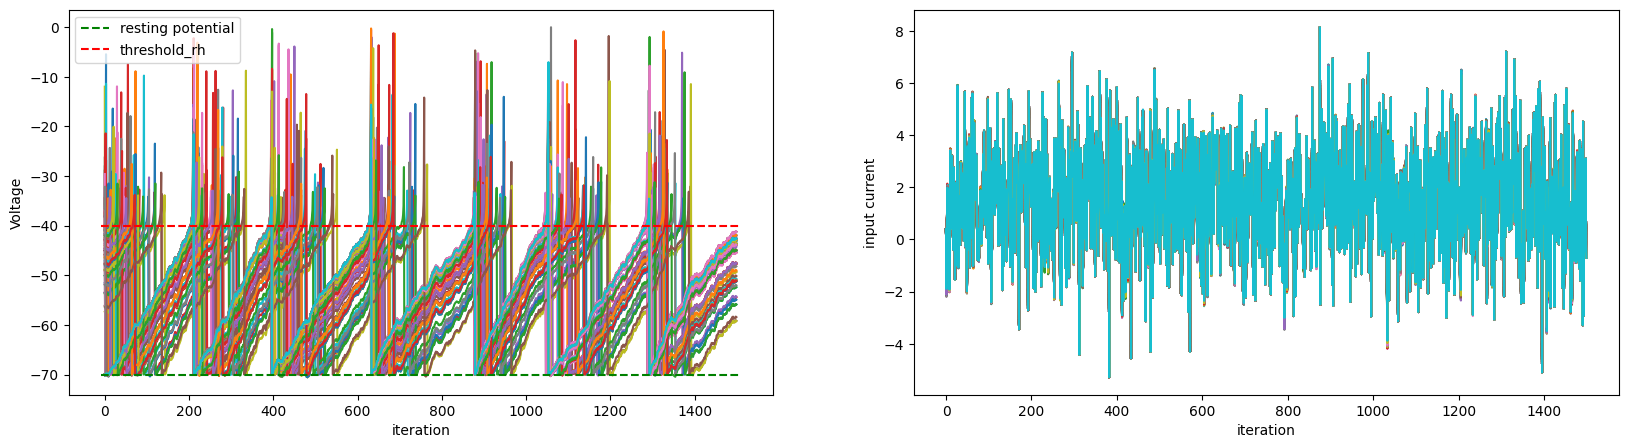
\includegraphics[width=\textwidth]{Figs/p-e.png}
    \caption{ نمودار جریان ورودی نویزی و تغییرات پتانسیل در جمعیت نورونی تحریکی}
  \end{subfigure}
  \\[\smallskipamount]
  \begin{subfigure}[b]{0.9\textwidth}
    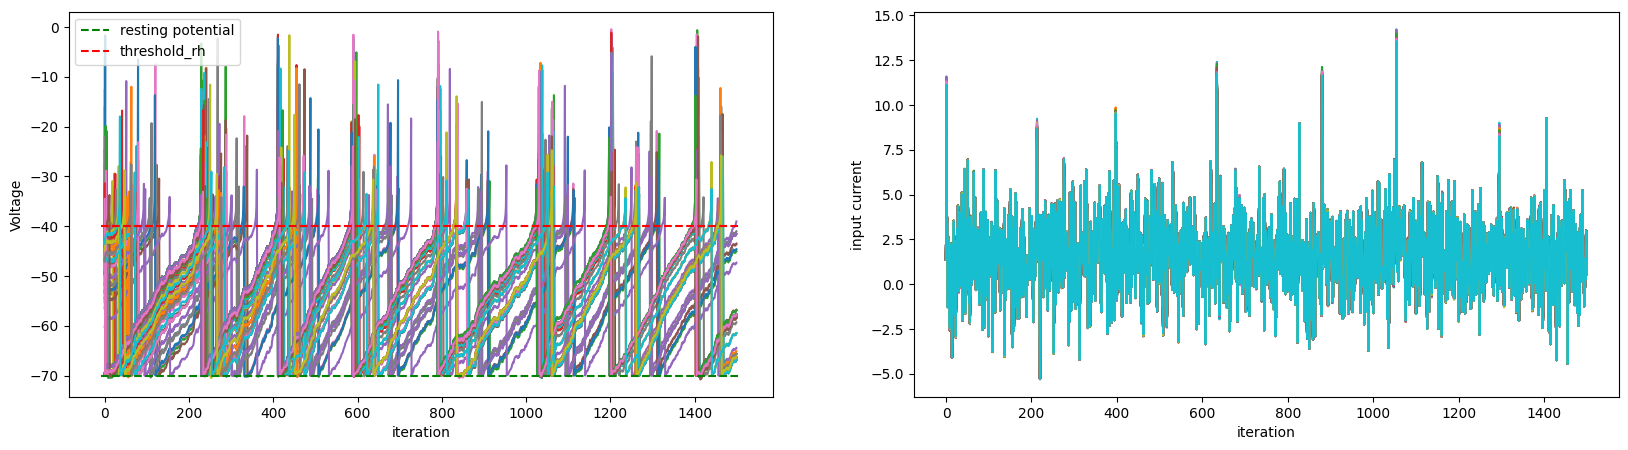
\includegraphics[width=\textwidth]{Figs/p-i.png}
    \caption{نمودار جریان ورودی نویزی و تغییرات پتانسیل در جمعیت نورونی مهاری}
  \end{subfigure}
  \caption{}
  \label{Fig:i-e}
\end{figure}
\end{center}

همانطور که در شکل \ref{Fig:i-e} مشاهده می‌کنید زمانی که فعالیت جمعیت مهاری ما افزایش می‌یابد به مرور اندکی کاهش در فعالیت جمعیت نورونی تحریکی رخ خواهد داد.


\begin{figure}[H]
\centering
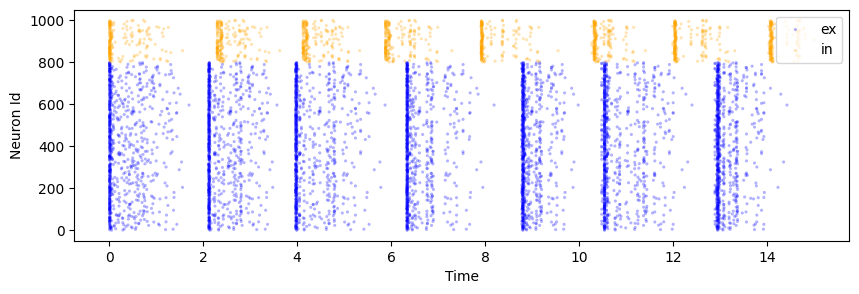
\includegraphics[width=0.8\textwidth]{Figs/raster1.png}
\caption{\lr{Raster plot} برای هر دو جمعیت مهاری و تحریکی }
\label{fig:raster1}
\end{figure}
\end{center}


با توجه به شکل \ref{fig:raster1} که \lr{Raster plot} را برای دو جمعیت نورنی مهاری و تحریکی نشان می‌دهد، که بعد از فعالیت در جمعیت‌های نورونی تحریکی به مرور فعالیت نورون‌های مهاری بیشتر می‌شود و با افزایش فعالیت نورون‌های مهاری فعالیت جمعیت نورونی تحریکی کمتر می‌شود.

	\subsection{ بررسی تاثیر پارامتر‌ها}
مانند قسمت قبل جمعیت‌های نورونی مهاری و تحریکی را با همان مشخصات و تعداد ایجاد می‌کنیم و میان آن‌ها از الگو‌های متفاوت برای برقراری ارتباط استفاده ‌می‌کنیم و \lr{Raster Plot} را برای هر کدام از آن‌ها رسم می‌کنیم.


\begin{figure}[H]
\centering
  \begin{subfigure}[b]{0.8\textwidth}
    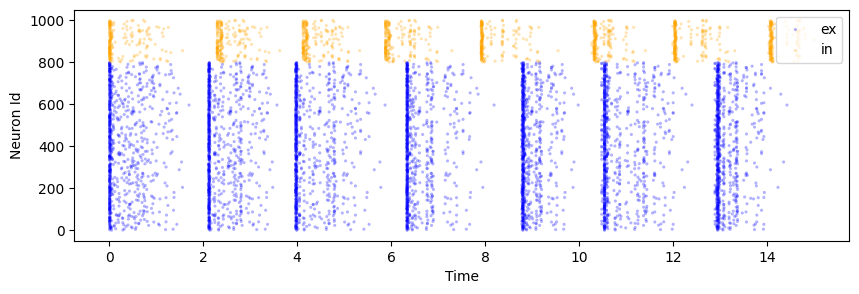
\includegraphics[width=\textwidth]{Figs/raster-f.png}
    \caption{\lr{full connectivity schema}}
  \end{subfigure}
  \\[\smallskipamount]
  \begin{subfigure}[b]{0.8\textwidth}
    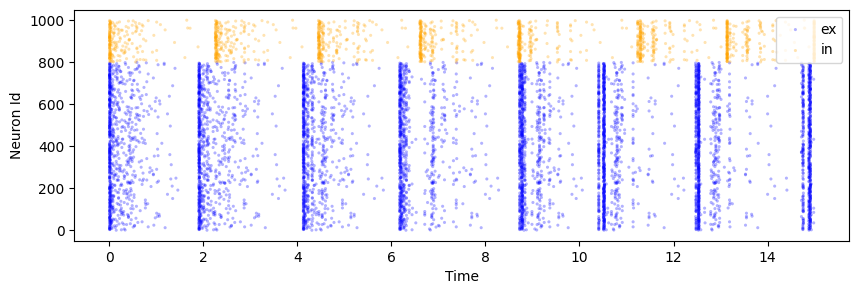
\includegraphics[width=\textwidth]{Figs/raster-prob.png}
    \caption{\lr{fixed coupling probability}}
  \end{subfigure}
  \\[\smallskipamount]
  \begin{subfigure}[b]{0.8\textwidth}
    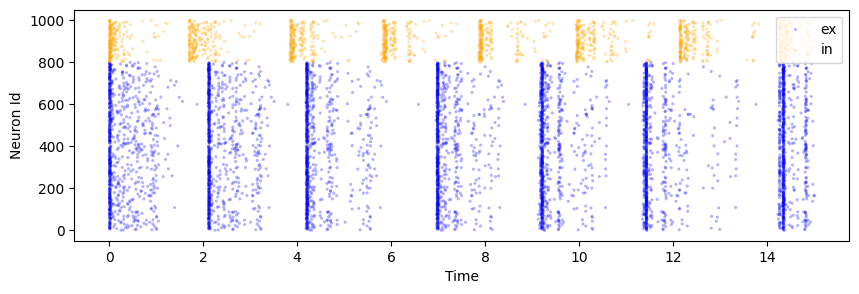
\includegraphics[width=\textwidth]{Figs/raster-count.png}
    \caption{\lr{fixed number of presynaptic partners}}
  \end{subfigure}
  \caption{}
  \label{Fig:f-p-c}
\end{figure}
\end{center}
	همانطور که در شکل \ref{Fig:f-p-c} مشاهده می‌کنید، زمانی که از الگوی ارتباطی کامل استفاده می‌کنیم بیشترین تراکم را در قسمت‌هایی که ضربه زده می‌شود داریم اما در حالتی که از حالت تعداد نورون‌های پیشین ثابت استفاده کرده‌ایم کمترین تراکم را داشته‌ایم و پراکندگی بیشتری مشاهده می‌شود، همچنین زمانی که از الگوی ارتباطی \lr{fixed number of presynaptic partners} 
	استفاده کرده‌ایم تاثیر نورون‌های مهاری بر روی نورون‌های تحریکی به بیشنیه مقدار خود رسیده که به وضوح کاهش ضربه و افزایش بازه میان ضربه‌ها در تصویر دیده‌ می‌شود.
	
	
	
	\section{تصمیم‌گیری}
	
	\subsection{شبیه‌سازی تصمیم‌گیری با وجود دو انتخاب}
	در این بخض دو جمعیت نورونی تحریکی متشکل از ۸۰۰ نورون \lr{AELIF} و یک جمعیت نورونی مهاری متشکل از ۲۰۰ نورون \lr{AELIF} تشکیل می‌دهیم، که ارتباط میان‌ آن‌ها را با استفاده از الگوی کامل برقرار می‌کنیم، شماتیک آن را می‌توانید در شکل  \ref{fig:pic} مشاهده کنید.

\begin{figure}[H]
\centering
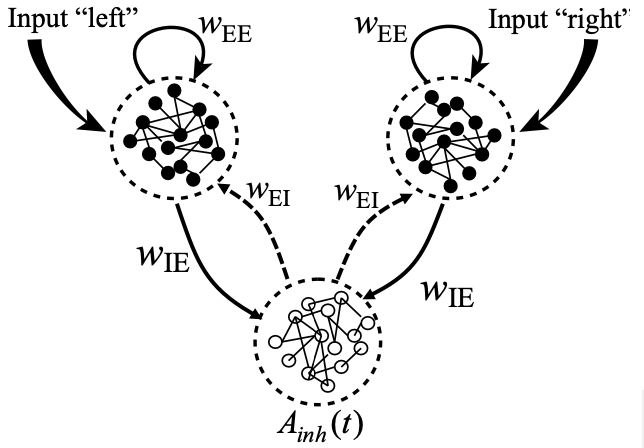
\includegraphics[width=0.4\textwidth]{Figs/pic.png}
\caption{شماتیک کلی جمعیت های نورونی ایجاد شده و ارتباطات میان آن‌ها}
\label{fig:pic}
\end{figure}
\end{center}

حال یک ورودی قوی‌تر را به جمعیت تحریکی دوم می‌دهیم تا در تصمیم گیری آن انتخاب شود، می‌توان نمودار تغییرات پتانسیل هر سه جمعیت را  در شکل \ref{Fig:e-e-i} مشاهده کرد، این نمودار نشان می‌دهد بعد از مدتی جمعیت نورونی تحریکی اول که ورودی کوچکتری دارد فعالیتش کمتر می‌شود و توسط جمعیت نورونی مهاری مهار می‌شود به نوعی، اما جمعیت نورونی تحریکی دوم به فعالیت خود ادامه می‌دهد و تقویت هم می‌شود.

\begin{figure}[H]
\centering
  \begin{subfigure}[b]{0.4\textwidth}
    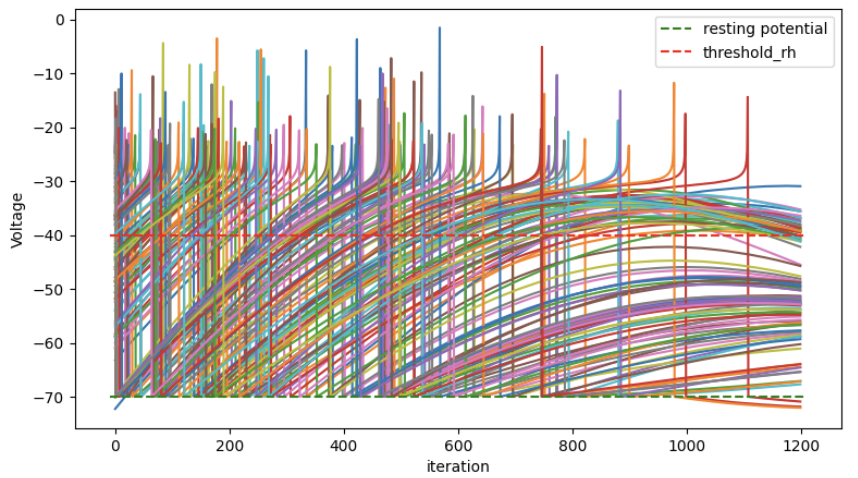
\includegraphics[width=\textwidth]{Figs/p-ex1}
    \caption{تغییرات پتانسیل جمعیت تحریکی اول}
  \end{subfigure}
  \hfill
  \begin{subfigure}[b]{0.4\textwidth}
    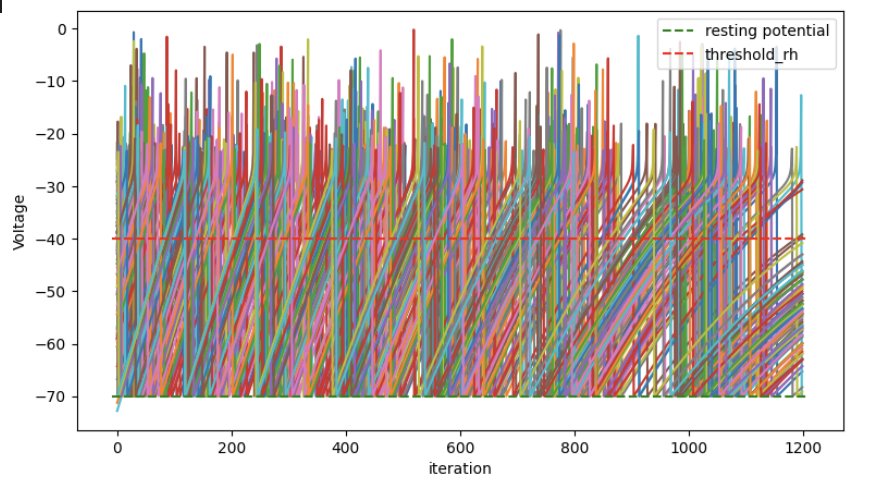
\includegraphics[width=\textwidth]{Figs/p-ex2}
    \caption{تغییرات پتانسیل جمعیت نورونی تحریکی دوم}
  \end{subfigure}
  \\[\smallskipamount]
  \begin{subfigure}[b]{0.4\textwidth}
    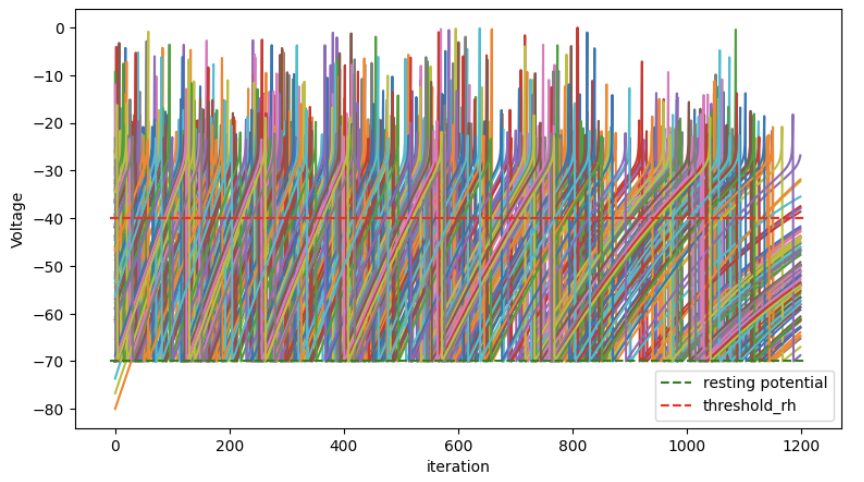
\includegraphics[width=\textwidth]{Figs/p-in}
    \caption{پتانسیل جمعیت نورونی مهاری}
  \end{subfigure}
  \caption{تغییرات پتانسیل جمعیت‌های نورونی متفاوت}
  \label{Fig:e-e-i}
\end{figure}
\end{center}

البته به این نکته باید توجه داشت که وقتی ما از مدل نورونی \lr{AELIF} استفاده کردیم فعالیت جمعیت ما لزوما بعد از مدتی به افزایش خود ادامه نخواهد داد و با توجه به خاصیت تطبیق پذیری که در نورون‌های ما وجود دارد فعالیت جمعیت کمتر می‌شود اما خب نسبت به جمعیت دیگر که در رقابت با آن پیروز شده است این اتفاق دیرتر رخ خواهد داد.

حال به صورت یکجا برای فعالیت هر سه جمعیت نورونی \lr{Raster plot} را رسم می‌کنیم شکل  \ref{fig:eei}، که مطابق انتظار جمعیت دوم با توجه به اینکه ورودی بزرگتری به آن وارد می‌شود به فعالیت خود ادامه می‌دهد اما جمعیت اول بازنده این رقابت می‌شود و از فعالیتش به مرور زمان کم می‌شود.


\begin{figure}[H]
\centering
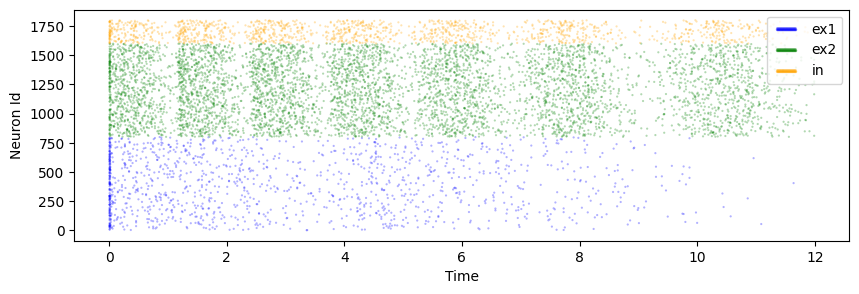
\includegraphics[width=0.9\textwidth]{Figs/raster-eei.png}
\caption{\lr{Raster Plot} برای دو جمعیت نورونی تحریکی و یک جمعیت مهاری}
\label{fig:eei}
\end{figure}
\end{center}

\subsection{بررسی تاثیر پارامترها}


\subsubsection{ اندازه جمعیت‌ها}
در این بخش آزمایش قبلی را با افزایش جمعیت نورونی مهاری تکرار می‌کنیم، همچنان دو جمعیت نورنی تحریکی با ۸۰۰ نورون خواهیم داشت اما یک جمعیت مهاری با ۸۰۰ نورون خواهیم داشت.

\begin{figure}[H]
\centering
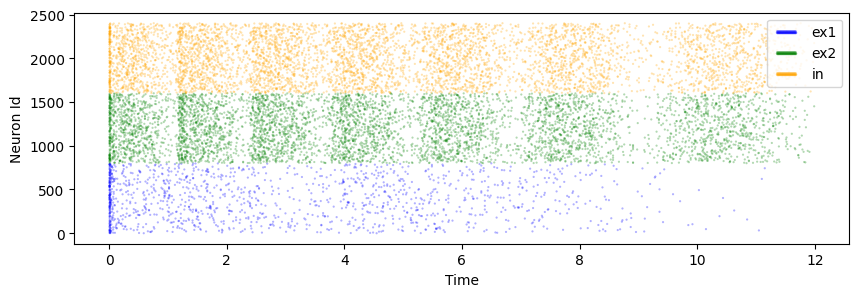
\includegraphics[width=0.9\textwidth]{Figs/raster3.png}
\caption{\lr{Raster Plot}  برای دو جمعیت نورونی تحریکی و یک جمعیت مهاری با ۸۰۰ نورون}
\label{fig:raster3}
\end{figure}
\end{center}

همانطور که در شکل \ref{fig:raster3} مشاهده می‌کنید، اینبار زمانی که ما تعداد نورون مهاری را بیشتر می‌کنیم سریع‌تر نورون های تحریکی جمعیت اول به نسبت فعالیتشان کاهش می‌یابد و از طرفی به طور کلی الگویی که میان فاصله هر دو اسپایک وجود داشت کاهش می‌یابد، زیرا  تعداد نورون‌های مهاری ما افزایش داشته و تاثیر منفی خواهند داشت در نتیجه بازه زمانی میان ضربه‌ها افزایش داشته است.

\subsubsection{الگوهای ارتباطی متفاوت}

	\begin{figure}[H]
\centering
  \begin{subfigure}[b]{0.8\textwidth}
    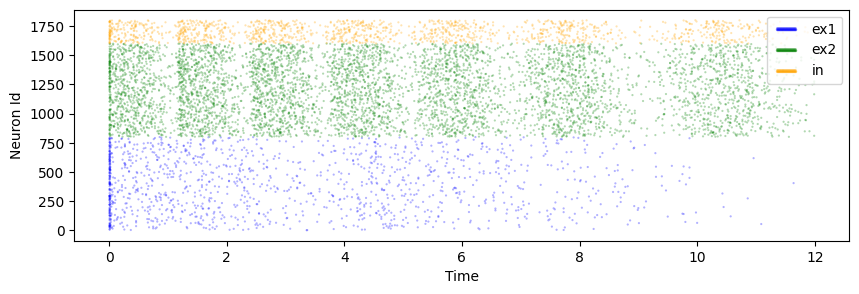
\includegraphics[width=\textwidth]{Figs/raster-eei.png}
    \caption{\lr{full connectivity schema}}
  \end{subfigure}
  \\[\smallskipamount]
  \begin{subfigure}[b]{0.8\textwidth}
    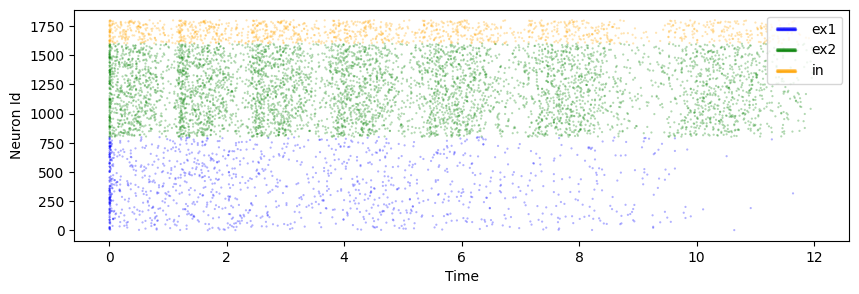
\includegraphics[width=\textwidth]{Figs/raster-prob1.png}
    \caption{\lr{fixed coupling probability}}
  \end{subfigure}
  \\[\smallskipamount]
  \begin{subfigure}[b]{0.8\textwidth}
    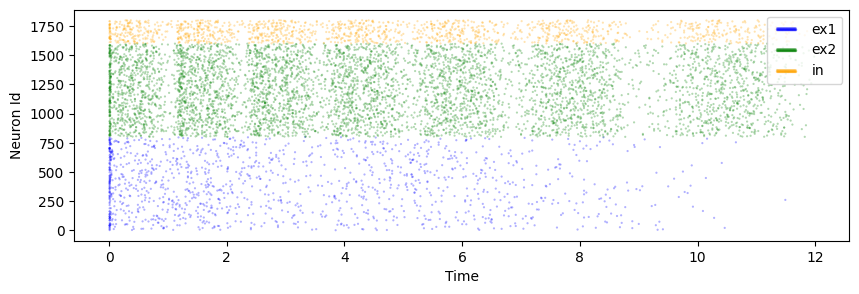
\includegraphics[width=\textwidth]{Figs/raster-count1.png}
    \caption{\lr{fixed number of presynaptic partners}}
  \end{subfigure}
  \caption{}
  \label{Fig:eei-p-c}
\end{figure}
\end{center}

در این بخش ما با استفاده از سه الگوی متفاوت میان جمعیت‌های نورونی اتصال ایجاد کردیم و نتیجه هر سه مدل در شرایط مشابه در شکل \ref{Fig:eei-p-c} مشاهده می‌شود، نکته‌ای که وجود دارد این است که به صورت کلی در رفتاری که ما در این بخش برای تصمیم گیری داریم تغییری ایجاد نمی‌شود چون آن جمعیتی که ورودی بزرگتری دارد در نهایت برنده این رقابت خواهد بود اگر اندازه وزن‌ها برابر باشد، بنابراین مطابق انتظار این مورد در رفتار نورون‌ها تغییری نداشته اما مثلا در جمعیت‌هایی که به صورت \lr{fixed coupling probability} به هم متصل هستند چون تعداد اتصالات کمتر بوده میزان فعالیت جمعیت‌ها نیز کمتر بوده است.


\section{نتیجه گیری}

همانطور که در این پروژه انتظار داشتیم جمعیت‌های نورونی را ساختیم و انواع الگوهای ارتباطی میان ‌آن‌ها را مورد بحث و تحلیل قرار دادیم، در نهایت نیز فرآیند تصمیم گیری در زمانی که دو انتخاب داشتیم را مورد بررسی قرار دادیم.

\end{document}